第一章习题(课本31页至34页)3 题,4 题 ,8 题 ,15 题 ,20 题 ,21 题 ,22 题 ,29 题 ,30 题。

\subsection{Questions}
\begin{statebox}{Question 3}{}
    Explain the difference between these two statements:
    \begin{itemize}
        \item \verb|result = 9*2|
        \item \verb|result = 9*2;|
    \end{itemize}
\end{statebox}
前者结尾有英文分号,表示不抑制结果输出,而后者则组织了结果输出。\footnote{The semicolon is used after an expression or statement to suppress printing. It is also used inside brackets to indicate the ends of the rows of a matrix.}


\begin{statebox}{Question 4}{}
    In what variable would the result of the following expression be stored:
    \begin{itemize}
        \item \verb|>> 3 + 5|
    \end{itemize}
\end{statebox}
\verb|ans| is the variable created automatically when expressions are not assigned to anything else. ANSwer. 因此结果存储在 \verb|ans| 变量中。


\begin{statebox}{Question 8}{}
    Find a format option that would result in the following output format:
    \begin{matlab}{}
>> 5/16 + 2/7
ans =
    67/112
    \end{matlab}
\end{statebox}
\begin{matlab}{}
>> help format
 format Set output format.
    format with no inputs sets the output format to the default appropriate
    for the class of the variable. For float variables, the default is
    format SHORT.
 
    format does not affect how MATLAB computations are done. Computations
    on float variables, namely single or double, are done in appropriate
    floating point precision, no matter how those variables are displayed. 
    Computations on integer variables are done natively in integer. Integer
    variables are always displayed to the appropriate number of digits for
    the class, for example, 3 digits to display the INT8 range -128:127.
    format SHORT and LONG do not affect the display of integer variables.
 
    format may be used to switch between different output display formats
    of all float variables as follows:
      format SHORT     Scaled fixed point format with 5 digits.
      format LONG      Scaled fixed point format with 15 digits for double
                       and 7 digits for single.
      format SHORTE    Floating point format with 5 digits.
      format LONGE     Floating point format with 15 digits for double and
                       7 digits for single.
      format SHORTG    Best of fixed or floating point format with 5 
                       digits.
      format LONGG     Best of fixed or floating point format with 15 
                       digits for double and 7 digits for single.
      format SHORTENG  Engineering format that has at least 5 digits
                       and a power that is a multiple of three
      format LONGENG   Engineering format that has exactly 16 significant
                       digits and a power that is a multiple of three.
 
    format may be used to switch between different output display formats
    of all numeric variables as follows:
      format HEX     Hexadecimal format.
      format +       The symbols +, - and blank are printed 
                     for positive, negative and zero elements.
                     Imaginary parts are ignored.
      format BANK    Fixed format for dollars and cents.
      format RAT     Approximation by ratio of small integers.  Numbers
                     with a large numerator or large denominator are
                     replaced by *.
 
    format may be used to affect the spacing in the display of all
    variables as follows:
      format COMPACT Suppresses extra line-feeds.
      format LOOSE   Puts the extra line-feeds back in.
 
    Example:
       format short, pi, single(pi)
    displays both double and single pi with 5 digits as 3.1416 while
       format long, pi, single(pi)
    displays pi as 3.141592653589793 and single(pi) as 3.1415927.
 
       format, intmax('uint64'), realmax
    shows these values as 18446744073709551615 and 1.7977e+308 while
       format hex, intmax('uint64'), realmax
    shows them as ffffffffffffffff and 7fefffffffffffff respectively.
    The HEX display corresponds to the internal representation of the value
    and is not the same as the hexadecimal notation in the C programming
    language.
 
    See also disp, display, isnumeric, isfloat, isinteger.

    Documentation for format
\end{matlab}
因此调用的格式修改为 \verb|format compact|。


\begin{statebox}{Question 15}{}
    Generate a random
    \begin{itemize}
        \item real number in the range (0, 30)
        \item real number in the range (10, 100)
        \item integer in the inclusive range from 1 to 20
        \item integer in the inclusive range from 0 to 20
        \item integer in the inclusive range from 30 to 80
    \end{itemize}
\end{statebox}
\begin{matlab}{}
30 * rand()
90 * rand() + 10
randi(20)
randi(21) - 1
randi(51) + 29
\end{matlab}


\begin{statebox}{Question 20}{}
    What would be the result of the following expressions?
    \begin{itemize}
        \item \verb|'b' >= 'c' - 1|
        \item \verb|3 == 2 + 1|
        \item \verb|(3 == 2) + 1|
        \item \verb|xor(5 < 6, 8 > 4)|
    \end{itemize}
\end{statebox}
\begin{matlab}{}
>> format compact
>> 'b' >= 'c' - 1
ans =
  logical
   1
>> 3 == 2 + 1
ans =
  logical
   1
>> (3 == 2) + 1
ans =
     1
>> xor(5 < 6, 8 > 4)
ans =
  logical
   0
\end{matlab}


\begin{statebox}{Question 21}{}
    Explain why the following expression results in 0 for false:
    \begin{itemize}
        \item 5>4>1
    \end{itemize}
\end{statebox}
两个大于号是顺序运行,因此先运算 \verb|5>4|,得到结果为布尔类型真,在 MATLAB 中布尔类型真在与双精度数值比较时会转化为双精度 \verb|1|,因此 \verb|1>1| 的结果为布尔类型假。


\begin{statebox}{Question 22}{}
    Explain why the following expression results in 1 for true:
    \begin{itemize}
        \item result = -20;
        \item 0 <= result <= 10
    \end{itemize}
\end{statebox}
两个小于等于号是顺序运行,因此先运算 \verb|0<=result|,得到结果为布尔类型假,在 MATLAB 中布尔类型假在与双精度数值比较时会转化为双精度 \verb|0|,因此 \verb|0<=10| 的结果为布尔类型真。


\begin{statebox}{Question 29}{}
    Use \verb|help elfun| or experiment to answer the following questions:
    \begin{itemize}
        \item Is \verb|fix(3.5)| the same as \verb|floor(3.5)|?
        \item Is \verb|fix(3.4)| the same as \verb|fix(-3.4)|?
        \item Is \verb|fix(3.2)| the same as \verb|floor(3.2)|?
        \item Is \verb|fix(-3.2)| the same as \verb|floor(-3.2)|?
        \item Is \verb|fix(-3.2)| the same as \verb|ceil(-3.2)|?
    \end{itemize}
\end{statebox}
\begin{matlab}{}
>> format compact
>> fix(3.5) == floor(3.5)
ans =
  logical
   1
>> fix(3.4) == fix(-3.4)
ans =
  logical
   0
>> fix(3.2) == floor(3.2)
ans =
  logical
   1
>> fix(-3.2) == floor(-3.2)
ans =
  logical
   0
>> fix(-3.2) == ceil(-3.2)
ans =
  logical
   1
\end{matlab}


\begin{statebox}{Question 30}{}
    \begin{itemize}
        \item For what range of values is the function \verb|round| equivalent to the function \verb|floor|?
        \item For what range of values is the function \verb|round| equivalent to the function \verb|ceil|?
    \end{itemize}
\end{statebox}
由函数定义或实验,我们可以根据符号与小数位(非负,例如 -1.2 的小数位为 0.2)判断是否等价,我们可以得出:
\begin{itemize}
    \item 如果为正,
        \begin{itemize}
            \item 如果小数位小于 0.5:\verb|round| 等价于 \verb|floor|;
            \item 如果小数位大于等于 0.5:\verb|round| 等价于 \verb|ceil|。
        \end{itemize}
    \item 如果为负,
        \begin{itemize}
            \item 如果小数位小于 0.5:\verb|round| 等价于 \verb|ceil|;
            \item 如果小数位大于等于 0.5:\verb|round| 等价于 \verb|floor|。
        \end{itemize}
\end{itemize}
其中,\verb|floor| 与 \verb|ceil| 在非整数点上均不等价。
\[
    \texttt{round}(x) = \begin{cases}
        \texttt{floor}(x), & x\in(n,n+\frac{1}{2})\text{ for }x\in\mathbb{Z}; \\
        \texttt{ceil}(x),  & x\in[n-\frac{1}{2},n)\text{ for }x\in\mathbb{Z}; \\
        \text{\texttt{floor}$(x)$ 与 \texttt{ceil}$(x)$ 均可} & x\in\mathbb{Z}.
    \end{cases}
\]
\begin{matlab}{}
figure;
hold on;

x = linspace(-1, 1);
scatter(x, round(x)==floor(x));
scatter(x, round(x)==ceil(x));

legend('round(x)==floor(x)', 'round(x)==ceil(x)')
\end{matlab}
\begin{center}
    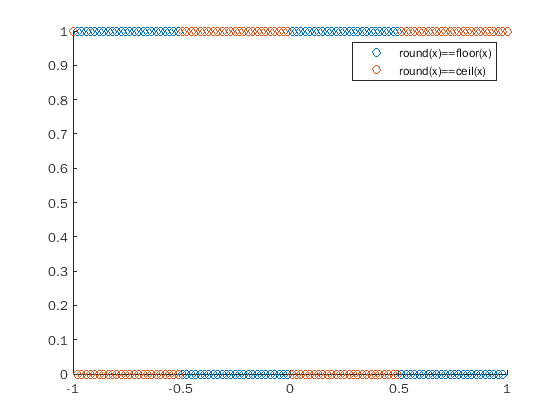
\includegraphics[width=.7\textwidth]{figures/1-1}
\end{center}
